\clearpage
\section{Video to Video via CogVideoX and CogVLM2-Caption}
\label{ap:v2v}

In this section, we present several examples of video-to-video generation using CogVideoX and CogVLM2-Caption. Specifically, we first input the original video into CogVLM2-Caption to obtain the video's caption, and then feed this caption into the CogVideoX model to generate a new video. From the examples below, it can be seen that our pipeline achieves a high degree of fidelity to the original video, showing that CogVLM2-Caption can capture almost all the details in the video.

\begin{figure}[h]
\begin{center}
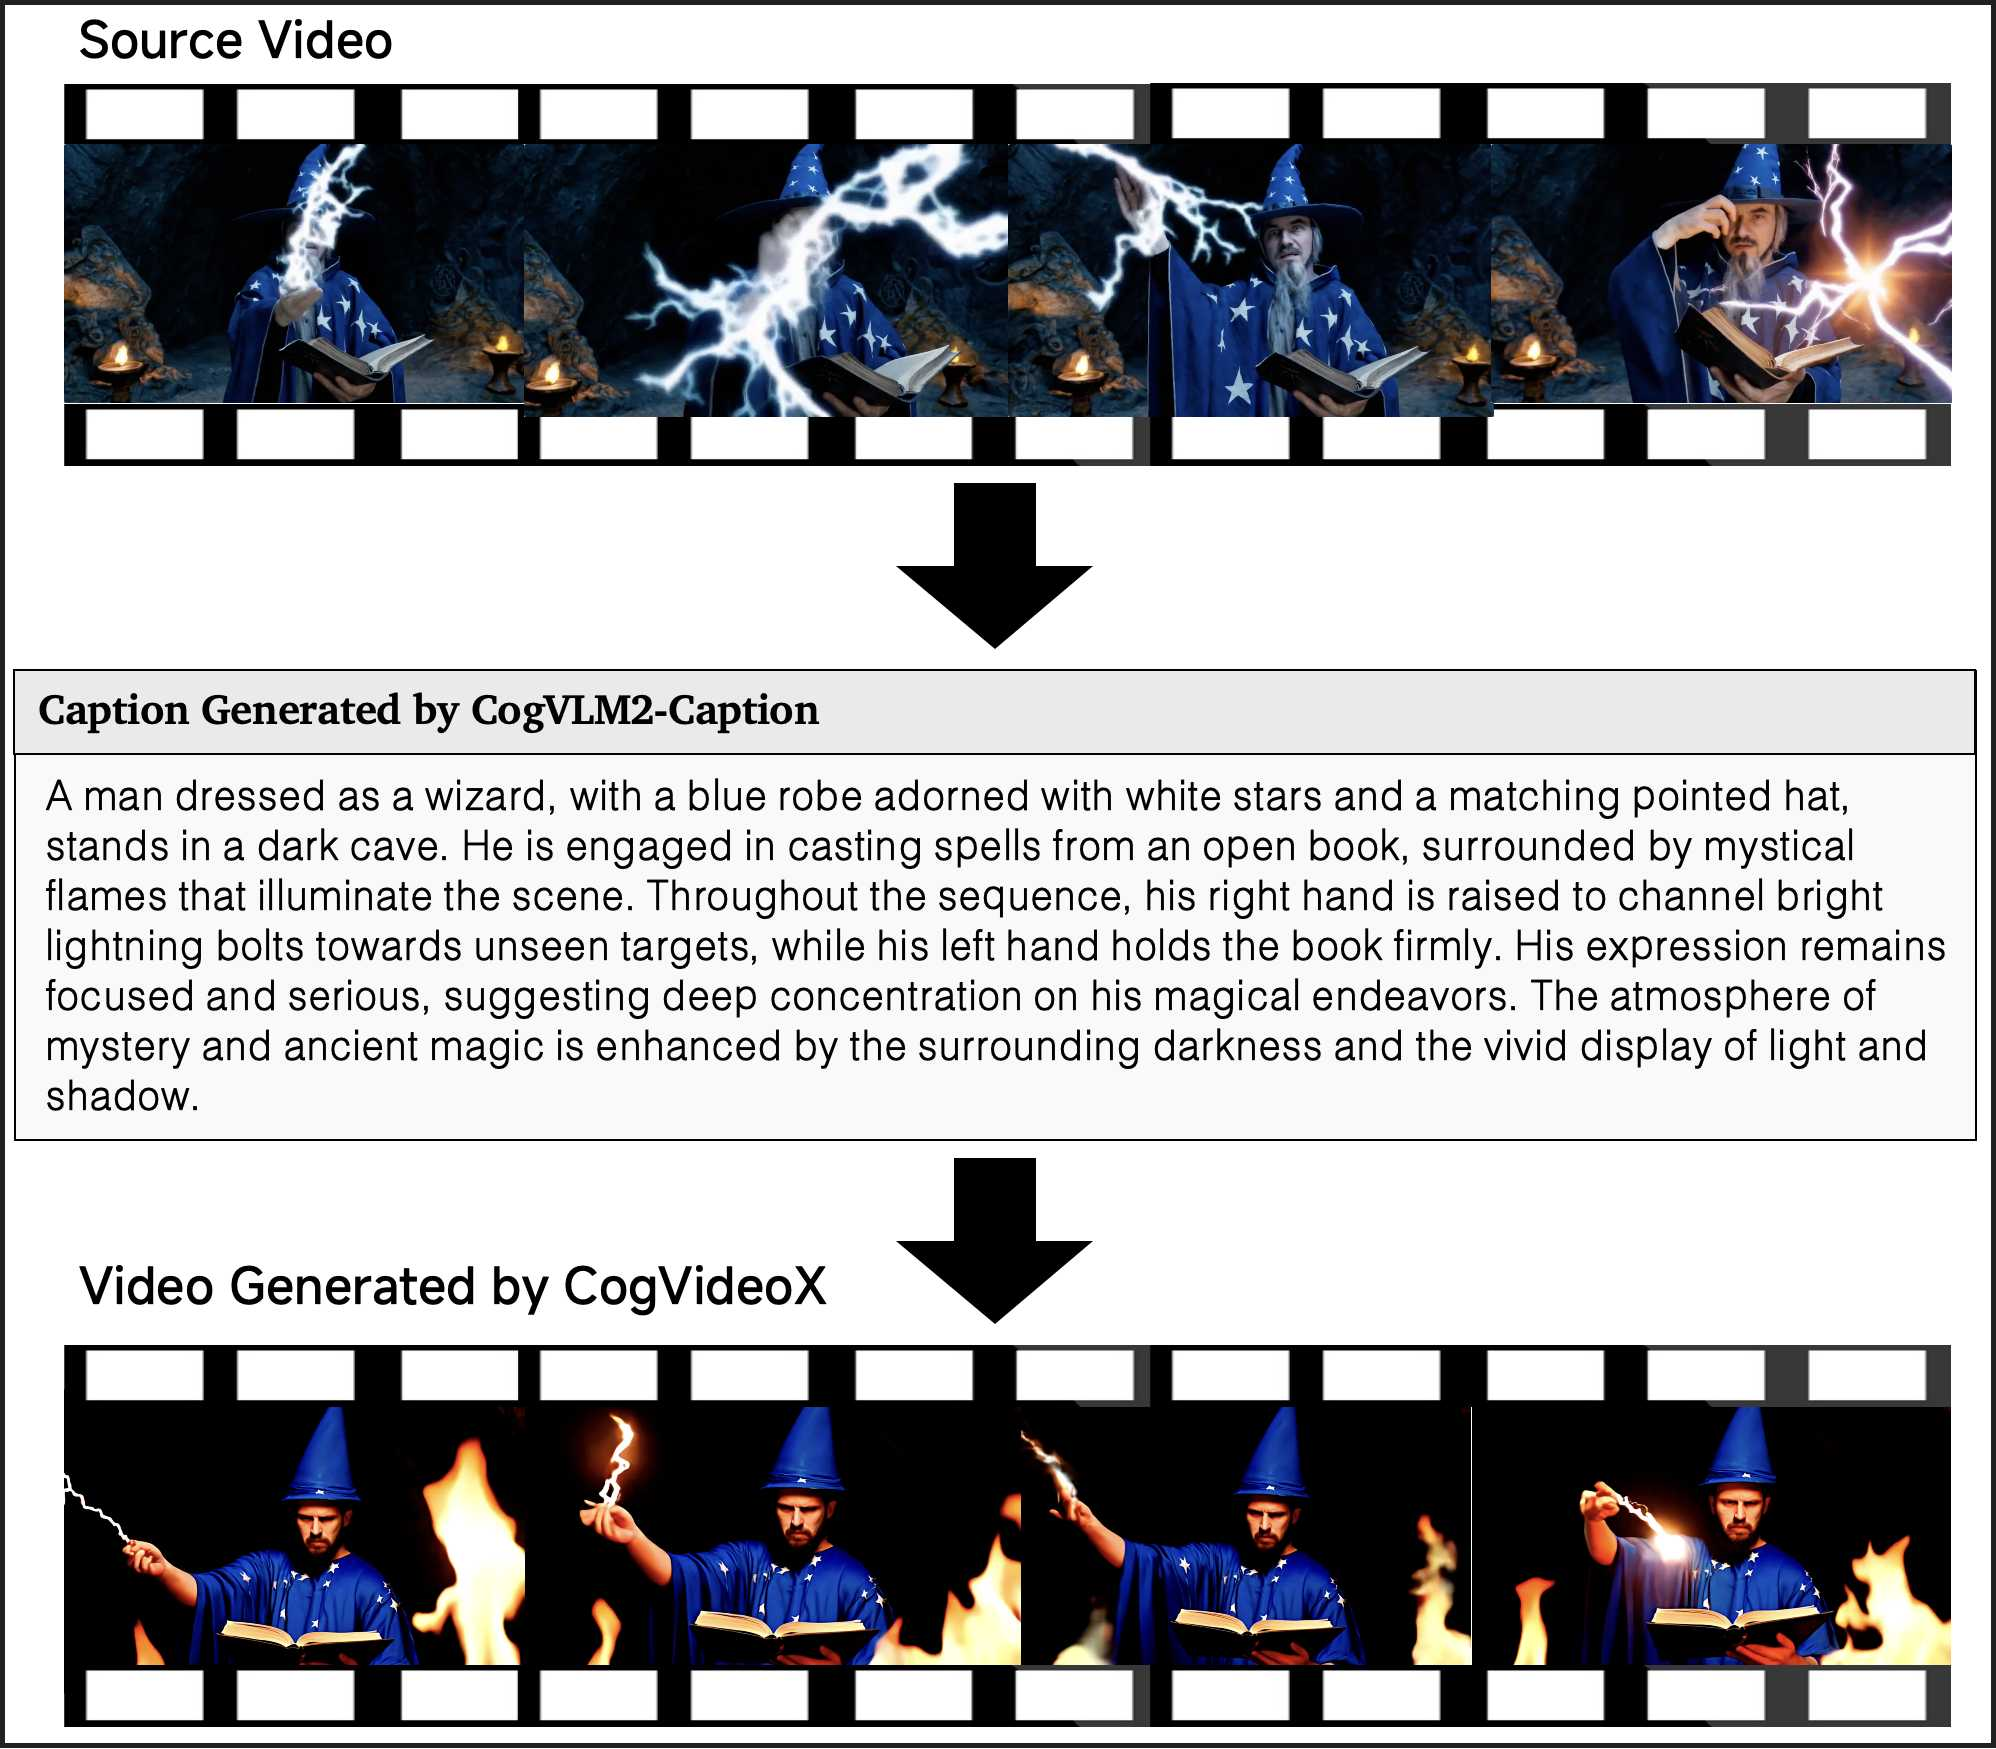
\includegraphics[width=0.9\linewidth]{images/v2v/v2v_1.jpg}
\end{center}
\end{figure}

\begin{figure}[h]
\begin{center}
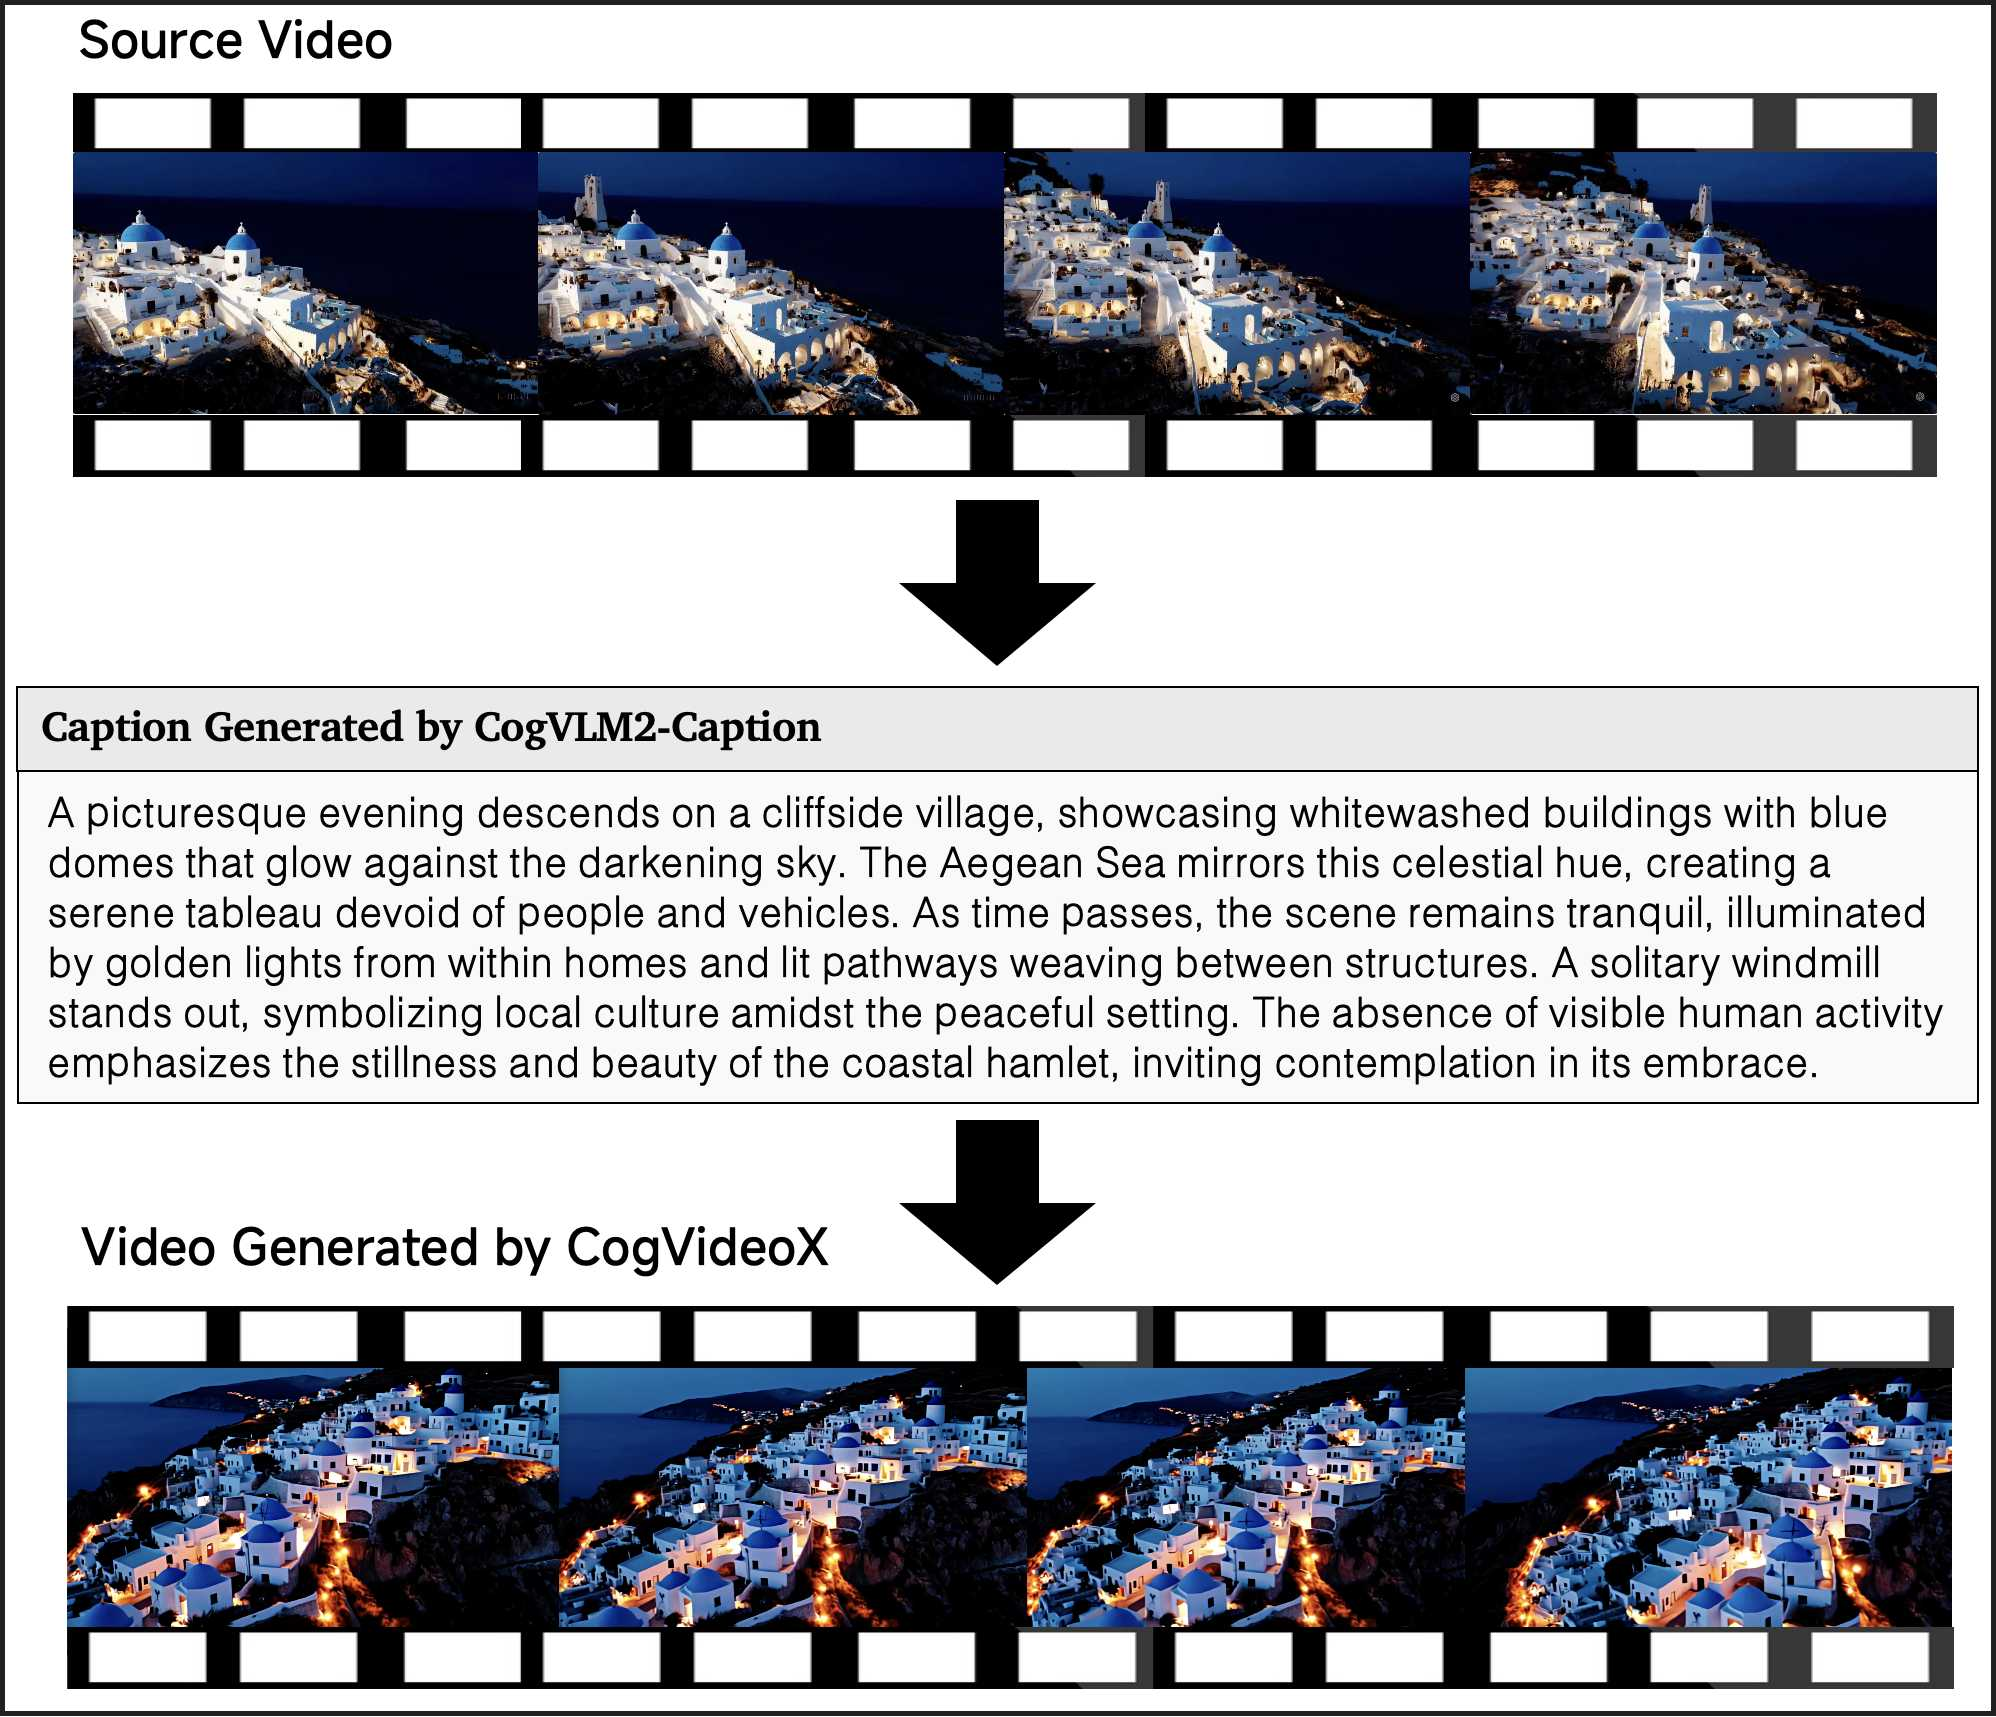
\includegraphics[width=0.9\linewidth]{images/v2v/v2v_2.jpg}
\end{center}
\end{figure}

\begin{figure}[h]
\begin{center}
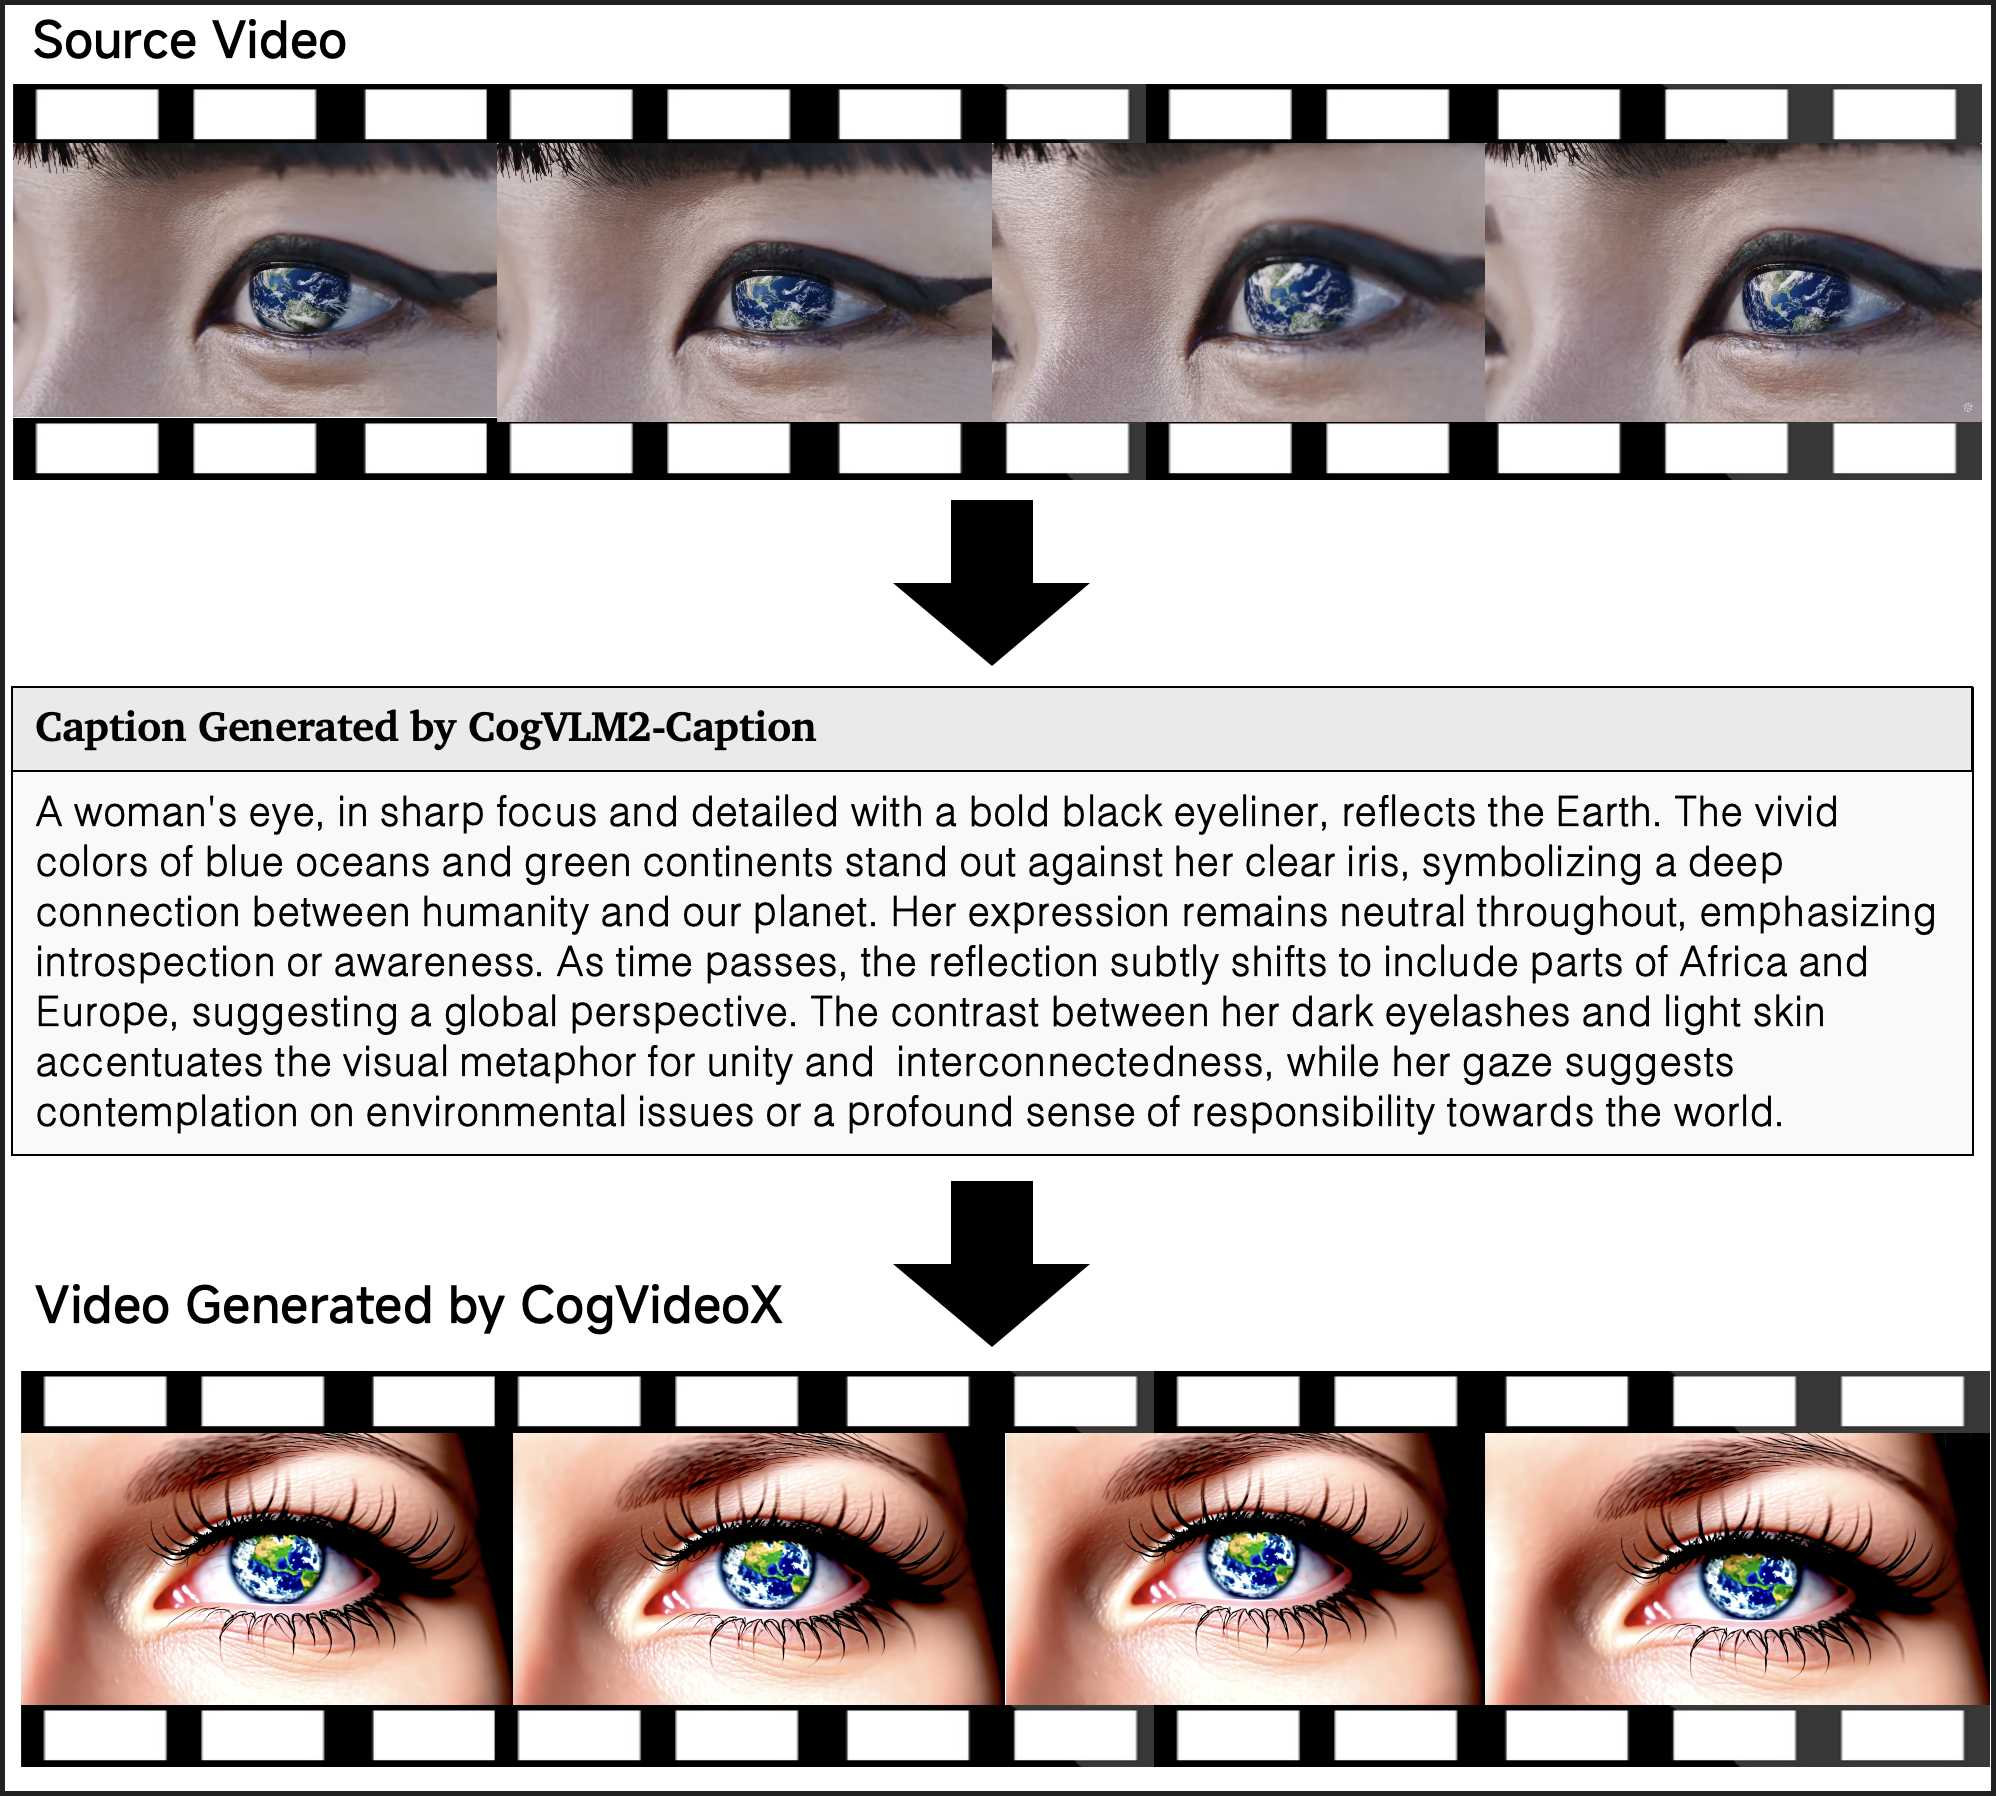
\includegraphics[width=0.9\linewidth]{images/v2v/v2v_3.jpg}
\end{center}
\end{figure}

